\documentclass[conference]{IEEEtran}
\usepackage[utf8]{inputenc}
\usepackage[T1]{fontenc}
\usepackage[spanish,es-noshorthands]{babel}
\usepackage{graphicx}
\usepackage{booktabs}
\usepackage{amsmath}
\usepackage{url}
\graphicspath{{figures/}{../figures/}}

% Manejo de floats: permitir paginas con mas figuras/tablas y evitar que se
% acumulen al final del documento.
\renewcommand{\topfraction}{0.92}
\renewcommand{\bottomfraction}{0.85}
\renewcommand{\textfraction}{0.07}
\renewcommand{\floatpagefraction}{0.78}
\renewcommand{\dbltopfraction}{0.92}
\renewcommand{\dblfloatpagefraction}{0.78}
\setcounter{topnumber}{2}
\setcounter{bottomnumber}{2}
\setcounter{totalnumber}{4}
\setcounter{dbltopnumber}{2}

\title{Super resolución eficiente de imagen única:\\¿alcanza un modelo pequeño? FSRCNN residual y ensamble por simetrías frente a EDSR}

\author{
\IEEEauthorblockN{Axel Fritz \quad Santiago Bunge}
\IEEEauthorblockA{Departamento de Ingeniería, Universidad de San Andrés\\
afritz@udesa.edu.ar \quad sbunge@udesa.edu.ar}
}

\begin{document}
\maketitle

\begin{abstract}
Se aborda el problema de super resolución de imagen única mediante modelos convolucionales
de la familia SRCNN y FSRCNN, evaluados sobre los conjuntos Set5, Set14, BSD100 y Urban100 en
factores de escala 2, 3 y 4. Como aporte propio se introduce una variante de FSRCNN que predice
el residuo sobre la interpolación bicúbica y se complementa con un ensamble por simetrías en la
etapa de inferencia. Esta combinación supera a la versión base de FSRCNN en las tres escalas y
alcanza una calidad comparable a la de EDSR, una red cerca de setenta veces más grande, usando
una fracción de los parámetros. El trabajo también analiza el efecto del tamaño del conjunto de
entrenamiento sobre los modelos de mayor capacidad y el compromiso entre distorsión y percepción
al incorporar pérdidas perceptuales y adversarias.
\end{abstract}

\section{Introducción}
La super resolución de imagen única consiste en reconstruir una versión de alta resolución a
partir de una imagen de baja resolución. Es un problema mal condicionado, ya que al reducir el
tamaño de una imagen se pierde información que luego debe estimarse. Muchas imágenes de alta
resolución distintas pueden dar lugar a la misma imagen reducida, de modo que no existe una única
solución correcta y el modelo debe inferir el detalle ausente. Los métodos clásicos de
interpolación, como vecino más cercano, bilineal y bicúbico, ofrecen una solución rápida pero
producen bordes difusos y texturas pobres.

El trabajo de Dong et al. mostró que una red convolucional sencilla, SRCNN, supera a la
interpolación bicúbica, y su versión acelerada, FSRCNN, mejora la velocidad operando en el
espacio de baja resolución. Modelos posteriores como EDSR incrementan fuertemente la capacidad
y la calidad a costa de muchos más parámetros y mayor cómputo. La super resolución tiene
aplicaciones concretas en restauración de fotografías, imágenes satelitales y médicas, y en el
escalado de video en tiempo real, donde el costo computacional es tan relevante como la calidad.

En este informe se implementa una progresión de arquitecturas, desde SRCNN hasta EDSR, y se
propone una mejora propia sobre FSRCNN. El objetivo no es únicamente maximizar la calidad, sino
estudiar la relación entre calidad, tamaño del modelo y costo de inferencia. La pregunta que
guía el análisis es si un modelo pequeño, bien diseñado y bien explotado, puede competir con uno
mucho mayor. Las contribuciones del trabajo son tres. Primero, una variante residual de FSRCNN
que mejora la calidad sin agregar parámetros. Segundo, el uso de un ensamble por simetrías en
inferencia que aporta una ganancia adicional sin reentrenar. Tercero, un análisis del efecto del
tamaño del conjunto de entrenamiento sobre los modelos grandes, que muestra que la capacidad
adicional de EDSR solo rinde con suficientes datos.

\section{Método}
\subsection{Convención de evaluación}
Todas las métricas se calculan sobre el canal de luminancia Y en el espacio YCbCr, siguiendo la
convención de la literatura del área. Se utiliza la conversión a YCbCr al estilo de MATLAB, con
rango acotado entre 16 y 235, y se descarta un borde de tamaño igual al factor de escala antes de
medir, ya que esos píxeles son artefactos del agrandado. La calidad se reporta con PSNR y con el
índice de similitud estructural SSIM. Estas decisiones no son menores: medir sobre los tres
canales de color o sin descartar el borde produce valores de PSNR distintos que no se pueden
comparar con los publicados. Para garantizar que la medición es correcta se valida que el PSNR de
la interpolación bicúbica coincide con los valores publicados, lo que actúa como control previo a
cualquier comparación entre modelos.

\subsection{Arquitecturas}
Se entrenaron cuatro arquitecturas de capacidad creciente:

\begin{itemize}
  \item \textbf{SRCNN}: tres convoluciones aplicadas sobre la imagen previamente agrandada por
  interpolación bicúbica. Opera en alta resolución, por lo que resulta más lenta y costosa.
  \item \textbf{FSRCNN}: trabaja directamente en baja resolución y agranda al final mediante una
  capa de deconvolución. Su estructura combina una etapa de reducción de dimensión, varias capas
  de mapeo no lineal y una etapa de expansión, lo que la vuelve rápida y liviana, con cerca de
  trece mil parámetros. Constituye el modelo base.
  \item \textbf{FSRCNN residual}: variante propuesta en este trabajo, descrita más abajo.
  \item \textbf{EDSR}: red profunda formada por bloques residuales sin normalización por lotes y
  un agrandado final por reordenamiento de píxeles. Posee cerca de un millón de parámetros, dos
  órdenes de magnitud por encima del modelo base.
\end{itemize}

\subsection{Mejora propia}
La mejora propuesta tiene dos componentes. El primero es una conexión residual sobre la
interpolación bicúbica. En lugar de que la red reconstruya la imagen completa desde cero, predice
solamente el residuo que debe sumarse a la versión bicúbica:
\begin{equation}
\hat{y} = \text{bicúbica}(x) + f_\theta(x),
\end{equation}
donde $x$ es la imagen de baja resolución y $f_\theta$ la red. La interpolación bicúbica ya aporta
las zonas suaves y la estructura general de la imagen, que son la parte fácil del problema. Al
predecir solo el residuo, la red concentra su capacidad en los bordes y las texturas finas, que es
donde la interpolación falla. Esto facilita el aprendizaje, acelera la convergencia y mejora la
calidad sin agregar parámetros. La idea sigue el aprendizaje residual introducido en VDSR.

El segundo componente es un ensamble por simetrías en inferencia, conocido como self-ensemble. La
imagen se procesa en sus ocho orientaciones, que surgen de combinar cuatro rotaciones con un
espejo horizontal. Cada salida se devuelve a su orientación original aplicando la transformación
inversa y luego se promedian las ocho reconstrucciones. Como los errores que comete la red en cada
orientación son distintos, el promedio tiende a cancelarlos y mejora el PSNR sin necesidad de
reentrenar. El costo es multiplicar por ocho el número de evaluaciones, lo que se traduce en mayor
tiempo de inferencia.

\subsection{Funciones de pérdida}
Para el modelo base se compararon tres funciones de pérdida: el error absoluto medio L1, el error
cuadrático medio L2 y la pérdida de Charbonnier, que es una aproximación suave de L1 más robusta a
valores atípicos. Además, sobre EDSR en escala 4 se entrenaron dos variantes orientadas a la
percepción. La primera usa una pérdida perceptual que compara características intermedias de una
red VGG19 preentrenada, en lugar de comparar píxeles directamente. La segunda agrega un esquema
adversario al estilo de SRGAN, en el que un discriminador aprende a distinguir imágenes reales de
generadas y el generador aprende a engañarlo. Ambas buscan estudiar el compromiso entre distorsión
y percepción.

\subsection{Detalles de entrenamiento}
Los modelos se entrenaron con el optimizador Adam, tasa de aprendizaje inicial de $10^{-3}$,
parches de baja resolución de 24 por 24 píxeles y ocho mil parches por época, extraídos con
aumentos de datos por espejos y rotaciones. El modelo base se entrenó durante 150 épocas con lotes
de 64 muestras, mientras que EDSR usó lotes de 16 por su mayor tamaño. La variante de EDSR
entrenada con DIV2K usó una tasa de aprendizaje de $10^{-4}$ y 300 épocas. El entrenamiento se
realizó en una GPU T4 sobre la plataforma Kaggle.

\section{Conjuntos de datos}
El entrenamiento principal se realizó con \textbf{T91}, conjunto de 91 imágenes que es el estándar
de los trabajos originales de SRCNN y FSRCNN. De cada imagen se extraen parches, de modo que el
número efectivo de ejemplos de entrenamiento es mucho mayor que la cantidad de imágenes. Los pares
de baja y alta resolución se generan reduciendo la imagen original con interpolación bicúbica al
estilo de MATLAB, de modo que la degradación coincide con la usada en la evaluación y se evita un
desajuste entre entrenamiento y prueba.

Para estudiar el efecto del tamaño del conjunto sobre los modelos grandes se reentrenó EDSR con un
subconjunto de cerca de doscientas imágenes de \textbf{DIV2K}, que contiene imágenes de alta
resolución mucho mayores y más variadas que las de T91.

La evaluación se hizo sobre cuatro conjuntos de prueba estándar, Set5, Set14, BSD100 y Urban100,
en las versiones de pares de baja y alta resolución del repositorio SelfExSR. Set5 y Set14 son
conjuntos pequeños y clásicos, BSD100 reúne cien imágenes naturales variadas y Urban100, compuesto
por escenas urbanas con muchas líneas y estructuras repetitivas, es el más exigente. Las
referencias a los conjuntos se incluyen al final.

\section{Resultados}
La Tabla~\ref{tab:psnr} resume el PSNR sobre Set5 para los baselines y los modelos principales en
las tres escalas. Todos los modelos entrenados superan a los baselines de interpolación y a los
valores objetivo de la consigna, fijados en 34, 31 y 29 dB para escala 2, 3 y 4. La variante
residual mejora de manera consistente al modelo base, y el agregado del ensamble por simetrías
aporta una ganancia adicional que lleva al modelo pequeño por encima de EDSR en las tres escalas.

\begin{table}[!htb]
\caption{PSNR (dB) sobre Set5, canal Y. SE indica ensamble por simetrías.}
\label{tab:psnr}
\centering
\begin{tabular}{lccc}
\toprule
Método & x2 & x3 & x4 \\
\midrule
Bicúbica (baseline) & 33.68 & 30.41 & 28.43 \\
SRCNN & 36.37 & -- & 30.27 \\
FSRCNN & 36.11 & 32.19 & 30.09 \\
FSRCNN residual & 36.74 & 32.94 & 30.66 \\
\textbf{FSRCNN residual + SE} & \textbf{37.05} & \textbf{33.13} & \textbf{30.90} \\
EDSR (entrenado con T91) & 36.57 & 32.87 & 30.32 \\
EDSR (entrenado con DIV2K) & 37.00 & 33.01 & 30.71 \\
\midrule
Objetivo de la consigna & 34 & 31 & 29 \\
\bottomrule
\end{tabular}
\end{table}

La Tabla~\ref{tab:full} extiende la comparación al resto de los conjuntos de prueba en escala 4. La
ventaja del modelo residual con ensamble por simetrías se mantiene en los cuatro conjuntos,
incluido Urban100, que es el más difícil. Esto indica que la mejora no depende de un conjunto
particular sino que generaliza.

\begin{table*}[!t]
\caption{PSNR (dB) / SSIM sobre los cuatro conjuntos de prueba, factor de escala 4, canal Y.}
\label{tab:full}
\centering
\begin{tabular}{lcccc}
\toprule
Método & Set5 & Set14 & BSD100 & Urban100 \\
\midrule
Bicúbica (baseline) & 28.43 / 0.8232 & 26.09 / 0.7217 & 25.96 / 0.6857 & 23.14 / 0.6736 \\
FSRCNN & 30.09 / 0.8668 & 27.28 / 0.7651 & 26.74 / 0.7265 & 24.14 / 0.7257 \\
FSRCNN residual & 30.66 / 0.8811 & 27.69 / 0.7753 & 26.96 / 0.7339 & 24.56 / 0.7439 \\
\textbf{FSRCNN residual + SE} & \textbf{30.90 / 0.8850} & \textbf{27.81 / 0.7788} & \textbf{27.05 / 0.7367} & \textbf{24.66 / 0.7477} \\
EDSR (T91) & 30.32 / 0.8772 & 27.39 / 0.7714 & 26.79 / 0.7315 & 24.39 / 0.7389 \\
EDSR (DIV2K) & 30.71 / 0.8810 & 27.67 / 0.7756 & 26.95 / 0.7355 & 24.55 / 0.7457 \\
EDSR adversario (SRGAN) & 29.06 / 0.8283 & 26.57 / 0.7303 & 26.13 / 0.6950 & 23.82 / 0.7017 \\
\bottomrule
\end{tabular}
\end{table*}

Observando la Tabla~\ref{tab:full} en detalle, la diferencia entre el modelo pequeño y EDSR se
acentúa en Urban100, el conjunto con más estructuras finas y repetitivas. Allí el modelo residual
con ensamble por simetrías alcanza 24.66 dB frente a 24.55 dB de EDSR entrenado con DIV2K, lo que
refuerza que la ventaja no proviene de un conjunto particularmente favorable. En Set14 y BSD100 el
comportamiento es análogo, con mejoras de entre una y dos décimas de decibel sobre EDSR.

La Tabla~\ref{tab:params} reúne la cantidad de parámetros de cada arquitectura por factor de
escala. El salto entre el modelo base y EDSR es de casi dos órdenes de magnitud, lo que vuelve más
notable que el modelo pequeño alcance una calidad similar.

\begin{table}[!htb]
\caption{Cantidad de parámetros por arquitectura y factor de escala.}
\label{tab:params}
\centering
\begin{tabular}{lccc}
\toprule
Arquitectura & x2 & x3 & x4 \\
\midrule
FSRCNN y FSRCNN residual & 12.809 & 12.809 & 12.809 \\
EDSR & 776.705 & 961.345 & 924.417 \\
\bottomrule
\end{tabular}
\end{table}

La Tabla~\ref{tab:loss} muestra la ablación de la función de pérdida sobre FSRCNN en escala 2. La
pérdida L2 obtiene un PSNR levemente superior, lo que es esperable dado que optimiza directamente
el error cuadrático sobre el que se define el PSNR, mientras que L1 y Charbonnier dan resultados
muy cercanos entre sí.

\begin{table}[!htb]
\caption{Efecto de la función de pérdida (FSRCNN, Set5, x2).}
\label{tab:loss}
\centering
\begin{tabular}{lc}
\toprule
Pérdida & PSNR (dB) \\
\midrule
L1 & 36.11 \\
L2 & 36.41 \\
Charbonnier & 36.21 \\
\bottomrule
\end{tabular}
\end{table}

La Tabla~\ref{tab:cost} compara calidad y costo. El modelo residual tiene cerca de trece mil
parámetros, frente a casi un millón de EDSR. Sin ensamble por simetrías es el más veloz por un
margen amplio, con una calidad apenas inferior. Con el ensamble alcanza la mejor calidad, a costa
de un tiempo de inferencia mayor por las ocho pasadas. La ventaja en cantidad de parámetros se
mantiene en todos los casos y se traduce en menor uso de memoria y almacenamiento.

\begin{table}[!htb]
\caption{Calidad frente a costo (Set5, x2). Latencia medida en una GPU local.}
\label{tab:cost}
\centering
\begin{tabular}{lccc}
\toprule
Modelo & Parámetros & PSNR & ms/img \\
\midrule
FSRCNN residual & 12.809 & 36.74 & 0.9 \\
FSRCNN residual + SE & 12.809 & 37.05 & 21.8 \\
EDSR (T91) & 776.705 & 36.57 & 18.2 \\
EDSR (DIV2K) & 776.705 & 37.00 & 18.0 \\
\bottomrule
\end{tabular}
\end{table}

Las curvas de convergencia de la Figura~\ref{fig:conv} muestran que la variante residual no solo
alcanza un PSNR mayor sino que estabiliza antes que el resto. Las Figuras~\ref{fig:cual2}
y~\ref{fig:cual4} presentan comparaciones visuales en escala 2 y 4, donde se aprecia la
recuperación de bordes respecto de la interpolación bicúbica. La Figura~\ref{fig:eff} ubica a cada
modelo en el plano calidad contra latencia, donde se observa que el modelo pequeño domina la región
de bajo costo.

\begin{figure}[!htb]
\centering
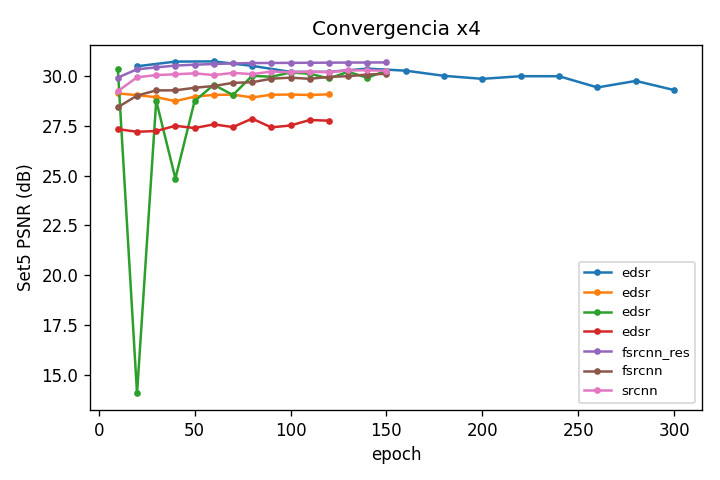
\includegraphics[width=\columnwidth]{convergencia_x4}
\caption{Curvas de convergencia (PSNR de validación sobre Set5) para el factor 4.}
\label{fig:conv}
\end{figure}

\begin{figure}[!htb]
\centering
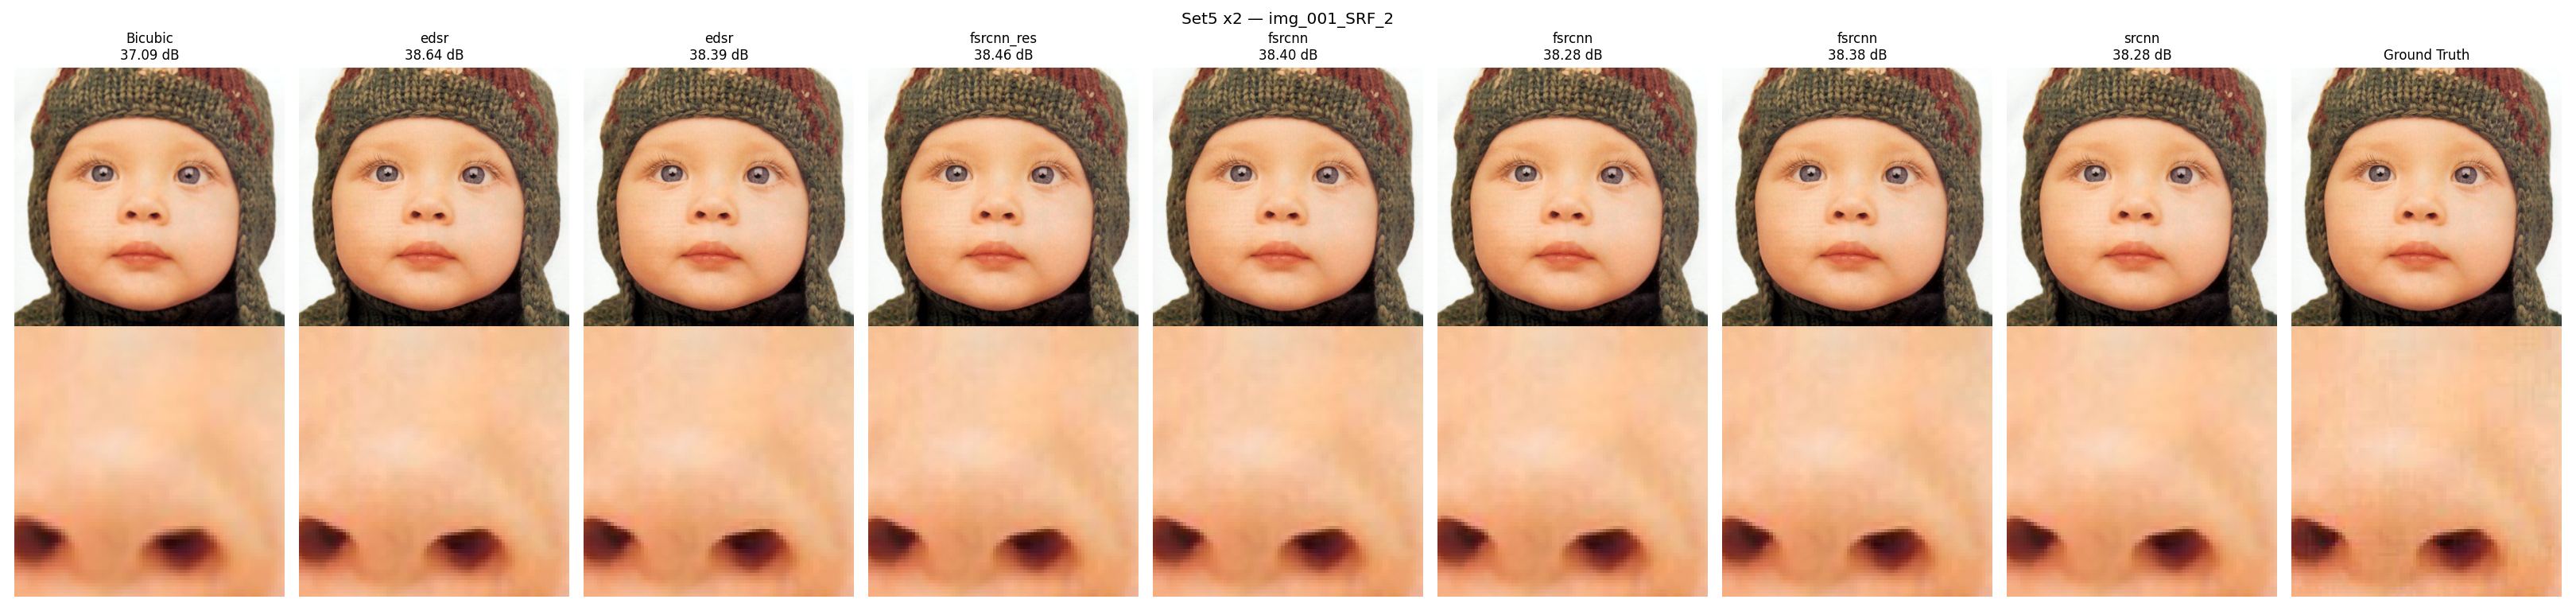
\includegraphics[width=\columnwidth]{cualitativo_Set5_x2_ej1}
\caption{Resultado cualitativo en Set5, escala 2.}
\label{fig:cual2}
\end{figure}

\begin{figure}[!htb]
\centering
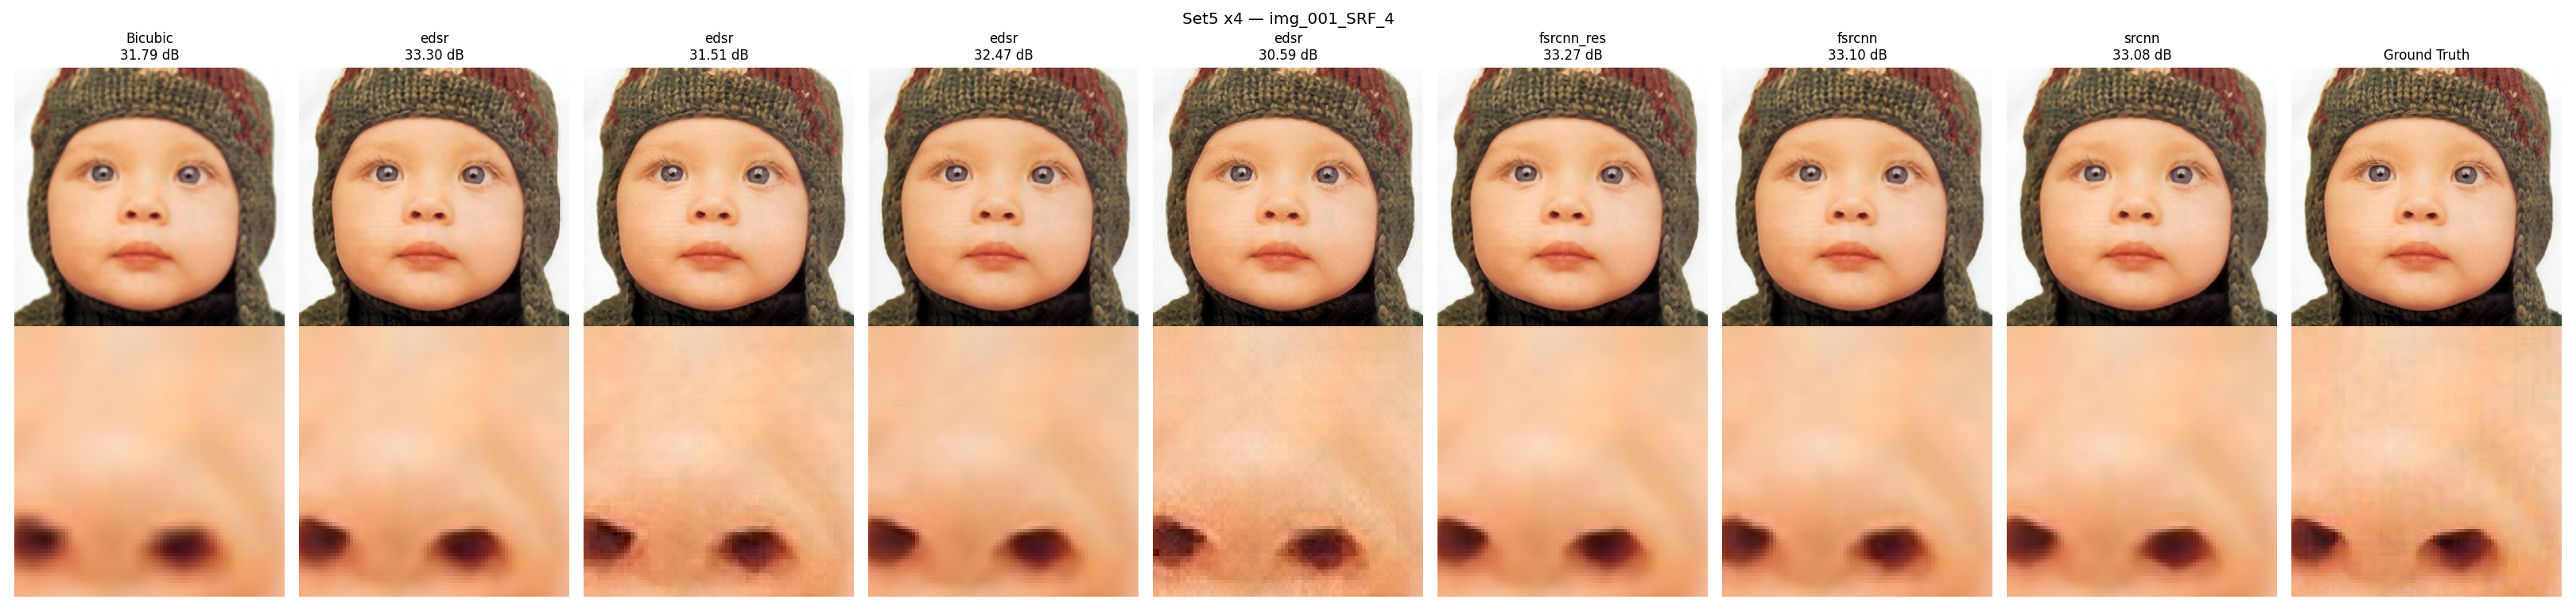
\includegraphics[width=\columnwidth]{cualitativo_Set5_x4_ej1}
\caption{Resultado cualitativo en Set5, escala 4. De izquierda a derecha, baja resolución,
bicúbica, modelos y referencia de alta resolución.}
\label{fig:cual4}
\end{figure}

\begin{figure}[!htb]
\centering
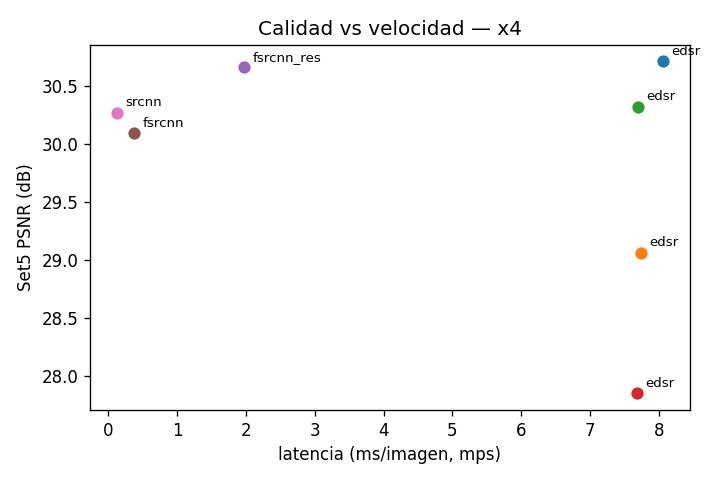
\includegraphics[width=\columnwidth]{eficiencia_x4}
\caption{Calidad frente a costo computacional por modelo en escala 4.}
\label{fig:eff}
\end{figure}

\section{Discusión}
Los resultados permiten varias lecturas. En primer lugar, la mejora propia cumple su objetivo. La
conexión residual sobre la interpolación bicúbica eleva el PSNR en las tres escalas sin sumar
parámetros, y el ensamble por simetrías agrega una mejora gratuita en términos de entrenamiento.
La combinación lleva al modelo base de 36.11 a 37.05 dB en escala 2, una ganancia cercana a un
decibel, y la ventaja se sostiene en los cuatro conjuntos de prueba.

En segundo lugar, el caso de EDSR ilustra que la capacidad sola no basta. Entrenado con las mismas
91 imágenes que el modelo pequeño, EDSR obtiene un PSNR menor, ya que su mayor cantidad de
parámetros no se aprovecha con tan pocos datos y tiende a desaprovechar su capacidad. Solo al
reentrenarlo con DIV2K logra superar a la versión básica del modelo pequeño, aunque sin alcanzar a
la variante con ensamble por simetrías. Esto sugiere que la elección entre un modelo grande y uno
pequeño no es independiente del presupuesto de datos disponible.

La Figura~\ref{fig:curves} ayuda a entender este comportamiento. Sobre T91, la curva de validación
de EDSR es marcadamente más ruidosa y oscila de una época a otra, y su mejor valor no supera al del
modelo residual pese a contar con sesenta veces más parámetros. La red grande tampoco logra una
pérdida de entrenamiento menor que la del modelo residual, de modo que su capacidad adicional no se
traduce ni en mejor ajuste ni en mejor generalización cuando los datos son escasos. La misma figura
permite comparar FSRCNN y su variante residual bajo condiciones idénticas de datos, pérdida y
configuración: el modelo residual mantiene una pérdida de entrenamiento más baja y un PSNR de
validación más alto durante todo el entrenamiento. Esto respalda que aprender el residuo entre la
imagen de alta resolución y la interpolación bicúbica es una tarea de optimización más sencilla que
reconstruir la imagen completa desde cero.

\begin{figure}[!htb]
\centering
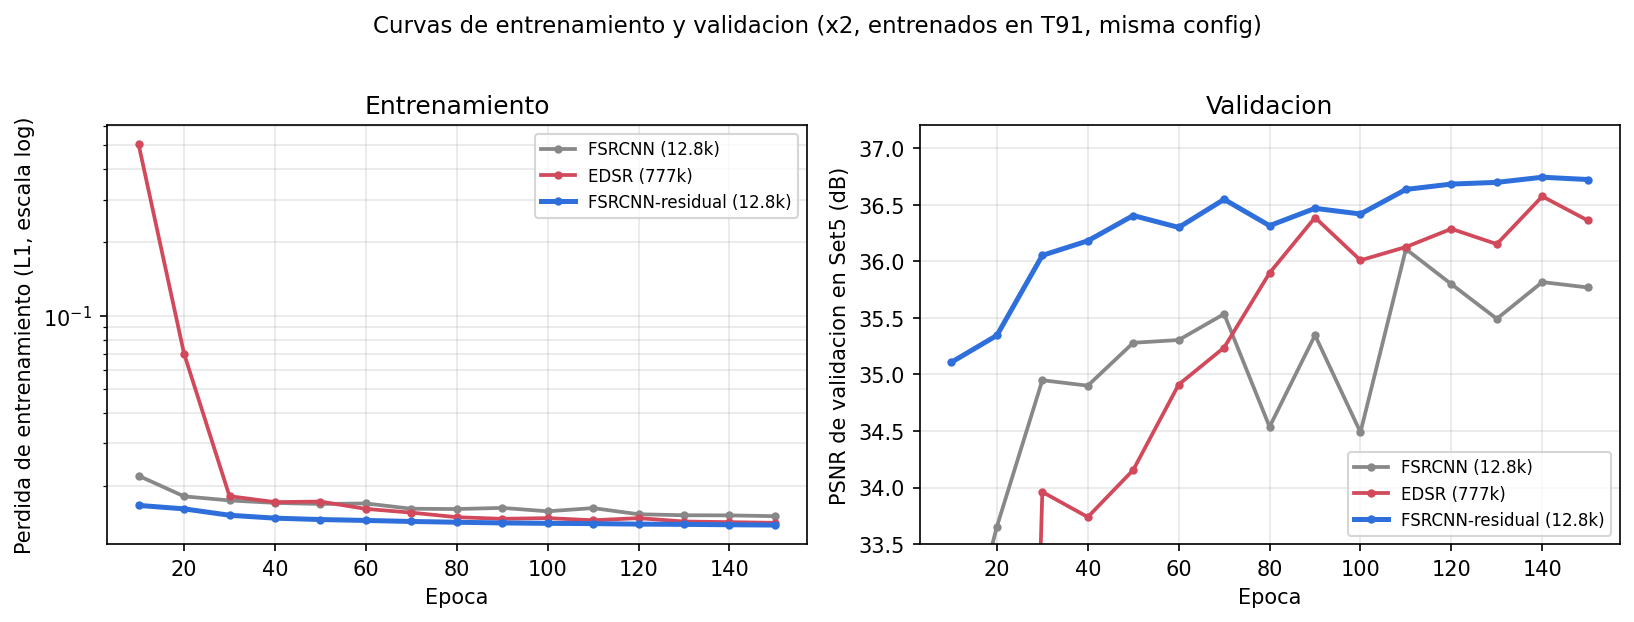
\includegraphics[width=\columnwidth]{curvas_train_val_x2}
\caption{Curvas de entrenamiento (pérdida L1, izquierda) y validación (PSNR sobre Set5, derecha) en
escala 2, para los tres modelos entrenados en condiciones idénticas sobre T91. El modelo residual
domina la validación de forma estable, mientras que EDSR resulta inestable y FSRCNN queda por debajo.}
\label{fig:curves}
\end{figure}

En tercer lugar, el análisis de costo muestra un compromiso claro. El modelo pequeño sin ensamble
es la mejor opción cuando interesa la velocidad, con una calidad apenas inferior. Con ensamble por
simetrías gana en calidad pero se vuelve más lento, dado que requiere ocho evaluaciones. Aun así,
mantiene una ventaja sólida en cantidad de parámetros frente a EDSR.

Por último, las variantes perceptual y adversaria confirman el compromiso entre distorsión y
percepción que muestra la Figura~\ref{fig:perc}. Estos modelos producen imágenes más nítidas pese a
un PSNR menor, lo que evidencia que el PSNR no captura por completo la calidad percibida y que una
mejora en la métrica no siempre equivale a una mejora visual.

\begin{figure}[!htb]
\centering
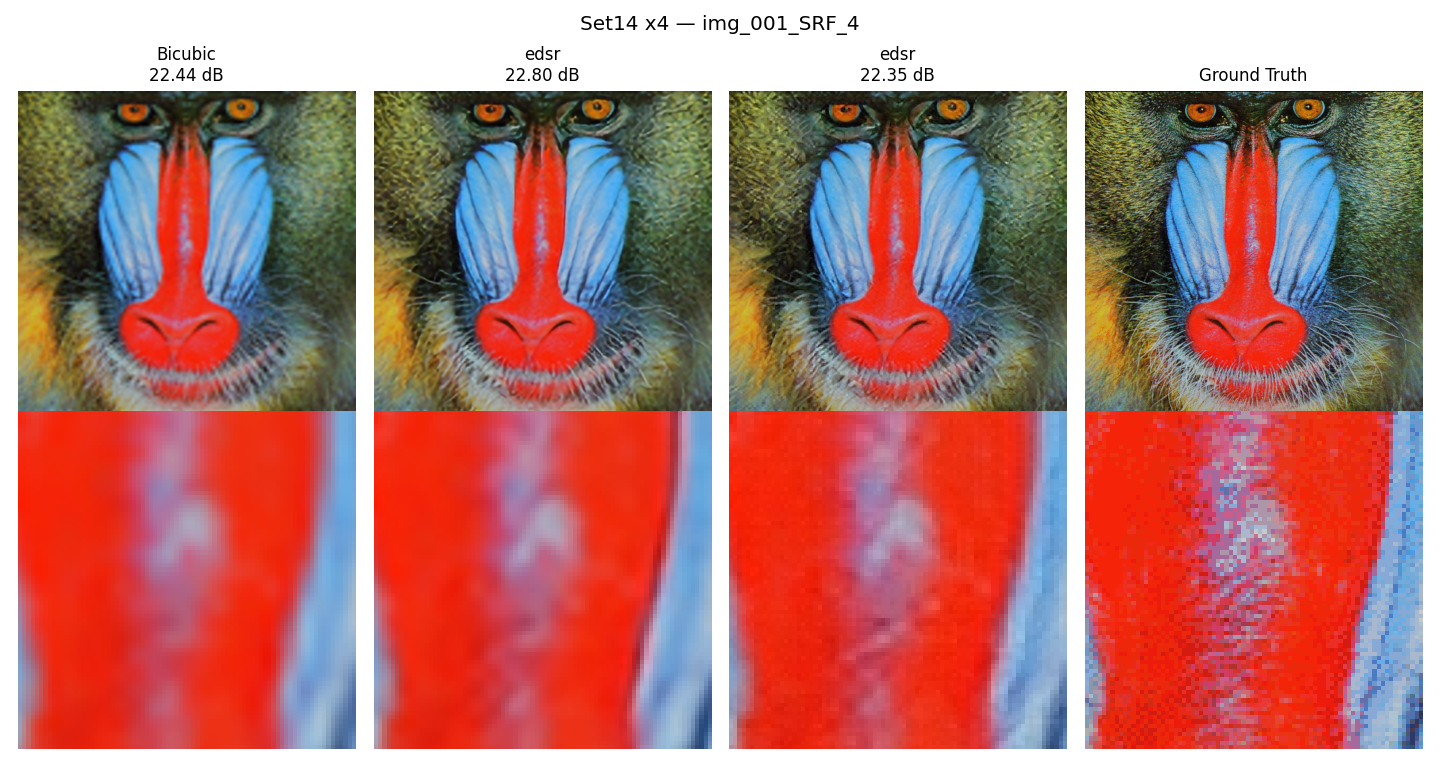
\includegraphics[width=\columnwidth]{percepcion_distorsion_x4}
\caption{Compromiso entre distorsión y percepción en escala 4. La variante adversaria genera
texturas más nítidas a pesar de un PSNR inferior.}
\label{fig:perc}
\end{figure}

\subsection{Trabajo a futuro}
Quedan abiertas varias líneas. Entrenar todos los modelos con un conjunto grande permitiría una
comparación pareja de arquitecturas, despejando el efecto de los datos. También sería de interés
aplicar el ensamble por simetrías a EDSR, explorar redes más profundas dentro de la familia FSRCNN
y evaluar con métricas perceptuales como LPIPS, que se correlacionan mejor con la percepción humana
que el PSNR.

\section*{Conclusión}
Se mostró que una red pequeña, FSRCNN con conexión residual y ensamble por simetrías, compite con
una red mucho mayor en super resolución de imagen única, superando los objetivos de la consigna en
las tres escalas y en los cuatro conjuntos de prueba con una fracción de los parámetros. El estudio
del tamaño del conjunto de entrenamiento y del compromiso entre calidad y costo aporta una mirada
útil para decidir qué modelo conviene según los recursos de datos y de cómputo disponibles.

\begin{thebibliography}{9}
\bibitem{srcnn} C. Dong, C. C. Loy, K. He y X. Tang, ``Image Super-Resolution Using Deep
Convolutional Networks,'' IEEE TPAMI, 2016.
\bibitem{fsrcnn} C. Dong, C. C. Loy y X. Tang, ``Accelerating the Super-Resolution Convolutional
Neural Network,'' ECCV, 2016.
\bibitem{vdsr} J. Kim, J. K. Lee y K. M. Lee, ``Accurate Image Super-Resolution Using Very Deep
Convolutional Networks,'' CVPR, 2016.
\bibitem{edsr} B. Lim, S. Son, H. Kim, S. Nah y K. M. Lee, ``Enhanced Deep Residual Networks for
Single Image Super-Resolution,'' CVPR Workshops, 2017.
\bibitem{srgan} C. Ledig et al., ``Photo-Realistic Single Image Super-Resolution Using a
Generative Adversarial Network,'' CVPR, 2017.
\bibitem{selfexsr} J.-B. Huang, A. Singh y N. Ahuja, ``Single Image Super-Resolution from
Transformed Self-Exemplars,'' CVPR, 2015. Conjuntos Set5, Set14, BSD100 y Urban100.
\bibitem{div2k} E. Agustsson y R. Timofte, ``NTIRE 2017 Challenge on Single Image
Super-Resolution: Dataset and Study,'' CVPR Workshops, 2017.
\end{thebibliography}

\end{document}
